\ylDisplay{Vardad} % Ülesande nimi
{Jaan Kalda} % Autor
{lahtine} % Voor
{2017} % Aasta
{G 10} % Ülesande nr.
{9} % Raskustase
{
% Teema: Dünaamika
\ifStatement
\begin{wrapfigure}[7]{r}{0.4\textwidth}
	\vspace{-10pt}
	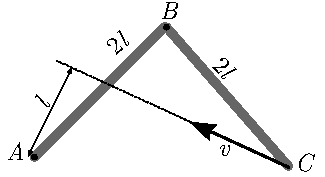
\includegraphics[width = 0.4\textwidth] {2017-lahg-10-delta.pdf}
\end{wrapfigure}

Juuresoleval joonisel on kujutatud kahest vardast pikkusega $2l$ koostatud \v sarniirne konstruktsioon. Ühe varda otspunkt on fikseeritud liikumatuna punkti $A$ ning teise varda otspunkt $C$ liigub konstantse kiirusega $v$ piki sihti, mis möödub punktist $A$ kaugusel $l$. Leidke varraste ühenduspunkti $B$ kiirendus hetkel, mil punktide $A$ ja $C$ vahekaugus on $2l$.
\fi


\ifHint
Punkti $B$ kiirust on võimalik leida, kasutades varraste venimatust ning asjaolu, et $A$ on fikseeritud. Punkti $B$ kiirenduse $AB$-sihilist komponenti saab leida kesktõmbekiirenduse kaudu ning kiirenduse suuna määramiseks on kasulik minna kiirusega $\vec{v}$ liikuvasse taustsüsteemi.
\fi


\ifSolution
Vaadeldaval hetkel on kiirusvektori ja $AC$ vahelise nurga siinus $\frac 12$, st nurk ise on $30^\circ$ ja seetõttu $AB$ on risti kiirusvektoriga. Järelikult on punkti $B$ kiirusvektori suund sama, mis $\vec v$. Varda $BC$ venimatuse tõttu peavad otspunktide kiirusvektorite projektsioonid varda sihile olema võrdsed. Et nurgad nende kiirusvektorite ja varda sihiga on võrdsed, siis peavad ka kiiruste moodulid olema võrdsed. Niisiis punkti $B$ kiirus on $\vec v$. Seetõttu on punkti $B$ kesktõmbekiirendus $v^2/2l$. Punktil $B$ võib olla veel mingi tangentsiaalkiirendus, hetkel me teame vaid kogukiirenduse projektsiooni $AB$ sihile. Läheme nüüd kiirusega $\vec v$ liikuvasse taustsüsteemi, kus punkt $C$ on kogu aeg paigal ja punkt $B$ on hetkeliselt paigal. Et $B$ on hetkeliselt paigal, siis selle kesktõmbekiirendus pöörlemisel ümber $C$ on antud hetkel null, st $B$ kiirenduse vektor on risti $BC$-ga. Seega me teame kiirenduse suunda ja projektsiooni $v^2/2l$ sihile $AB$ (mis moodustab vektori suunaga nurga $30^\circ$). Selle põhjal saame avaldada kiirenduse mooduli $a=v^2/(2l\cos30^\circ)=v^2/\sqrt 3l$.
\fi


\ifEngStatement
% Problem name: Rods
\begin{wrapfigure}[7]{r}{0.4\textwidth}
	\vspace{-10pt}
	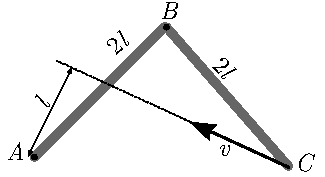
\includegraphics[width = 0.4\textwidth]  {2017-lahg-10-delta.pdf}
\end{wrapfigure}
In the given figure a hinged construction is pictured, it consists of two rods with a length $2l$. One of the rod’s tip is fixed to an unmoving point $A$ and the other rod’s tip $C$ moves with a constant velocity $v$ along a direction which passes the point $A$ at the distance $l$. Find the acceleration of the connection point $B$ of the rods during the moment when the distance between the points $A$ and $C$ is $2l$.
\fi


\ifEngHint
The velocity of the point $B$ is possible to find by using the non-stretchability of the rods and the fact that $A$ is fixed. The $AB$-directional acceleration component of the point $B$ can be found with centripetal acceleration. To determine the direction of the acceleration it is useful to go to the frame of reference of moving with the speed $\vec{v}$.
\fi


\ifEngSolution
The sine of the angle between velocity and $AC$ is $\frac 12$ at the moment of observation, meaning that the angle itself is $30^\circ$ and because of this $AB$ is perpendicular to the velocity. Therefore the direction of the point’s $B$ velocity is the same as $\vec v$. Due to the non-stretchability of the rod $BC$ the projections of the velocities on the rod’s ends have to be the same on the rod’s direction. Because the angles between these velocities and the direction of the rod are equal then the modules of the velocities have to be equal as well. Thus, the velocity of the point $B$ is $\vec v$. Because of this the centripetal acceleration of the point $B$ is $v^2/2l$. The point $B$ might also have some tangential acceleration, but at the moment we only know the projection of the total acceleration to the direction of $AB$. Let us now go to the velocity’s $\vec v$ frame of reference where the point $C$ is constantly still and the point $B$ momentarily still. Since $B$ is momentarily still then at the given moment its centripetal acceleration when rotating around $C$ is zero, meaning the acceleration vector of $B$ is perpendicular to $BC$. Therefore we know the direction of the acceleration and the projection of $v^2/2l$ to the direction of $AB$ (which forms the angle of $30^\circ$ with the direction of the vector). Based on this we can calculate the acceleration’s module $a=v^2/(2l\cos30^\circ)=v^2/\sqrt 3l$.
\fi
}